\section{Design of flexible batched \spmv kernels for GPUs}
\label{2017-batched-spmv:sec:s3-kerneldesign}

\subsection{Flexible batched \spmv}

A batched sparse \spmv for scientific applications often
comes with some boundary conditions, which allows optimizing the kernel
for this specific setting. Examples are situations where all \spmv operations of the batch have:
\begin{itemize}
\itemsep=0pt
\item
the same system size (which, as long as the sparsity pattern does not change too drastically,
allows to use explicit zero padding to fix the sparsity pattern);
\item
the same nonzero-per-row distribution 
(allows reuse of row pointers/row indices);
\item
the same nonzero locations
(allows reuse of row pointers/row indices and column indices);
\item
the same values but distinct sparsity patterns (allows reuse of the values);
\item
the same matrix scaled by a scalar
(which allows to rewrite the batched \spmv as a sparse matrix-matrix product and scaling the column of the distinct vectors).
\end{itemize}
In our case, we design our 
{\em flexible} kernels to tackle the most general case:
the systems can differ in size, nonzero count, nonzero distribution, and values. 
This solution offers greater flexibility, and even allows to process a batch of problems
coming from several concurrently-running applications.

\subsection{GPU kernel design}

A central aspect in the design of the batched kernels is the optimization of
the access to the vectors. For this purpose we initially read the vectors into
shared memory, which significantly reduces the cost of accessing them 
in the multiplication phase. As shared memory access is limited to the thread block,
it is a natural choice to assign one thread blocks to each problem of the matrix batch.
We design the batched \spmv kernels with focus on matrices of size up to 1,024 rows.
Technically it is possible to process also larger systems, 
but targeting batches containing small matrices makes this a reasonable design choice.

In this paper we implement and compare six kernels for processing
a batch of multiple {\spmv}s, with matrices stored in either CSR, COO or ELL format.
While the properties of the COO and ELL formats inherently result in
balanced workload distributions for each problem, we consider four implementations
for the CSR format that use different strategies to balance the work.

Currently, all implementations use one CUDA thread block per problem.
Thus, the same amount of resources, in terms of
shared memory and number of threads, is allocated to each problem in the batch.
We recognize this can result in workload imbalance in-between the distinct problems.
However, optimizing the resource allocation to the characteristics of the distinct matrices in the batch remains outside the scope of this work.

\begin{figure}[t]
\lstinputlisting[language=C]{codes/coo.c}
\lstinputlisting[language=C]{codes/csr.c}
\lstinputlisting[language=C]{codes/csr_i.c}
\lstinputlisting[language=C]{codes/ell.c}
\caption
[Sequential C implementations of basic \spmv algorithms]
{Sequential C implementations of basic \spmv algorithms.}
\label{2017-batched-spmv:fig:spmv}
\end{figure}

\subsection{COO}
The first listing 
in Figure~\ref{2017-batched-spmv:fig:spmv} (routine {\tt SpMV\_COO}) offers a sequential implementation 
of the \spmv kernel based on COO.
The natural approach to exploit hardware concurrency in this case
is to parallelize the loop traversing the nonzero elements in the matrix
(line~2 in the code). 
This strategy comes with two advantages: 1) the data access to the matrix
is coalescent; and
2) the workload
is perfectly balanced.
The disadvantage
is that multiple threads
may be assigned to elements located in the same row, and careful synchronization 
is necessary to ensure the partial sums are handled correctly. 
In order
to ensure correct synchronization,
in our batched implementation we combine atomic operations 
with thread-local partial sums. Moreover, each thread, typically handling multiple elements
located in the same row, does not write its partial sum to global memory until
all elements of the row are processed.
In addition, intra-warp atomic collisions are avoided
using warp-local segmented scans before each write.
In the remainder of the paper, we use the abbreviation \coo when referring to the
flexible batched \spmv routine based on COO.

\subsection{CSR}
A simple parallelization of \spmv based on CSR 
is obtained by mapping the distinct rows to different threads.
This corresponds to parallelizing the outer for-loop in the second listing
in Figure~\ref{2017-batched-spmv:fig:spmv} ({\tt SpMV\_CSR}).
This variant was first described for GPUs in~\cite{garlandspmv},
under the name CSR-scalar.
Even though CSR-scalar does not require any synchronization,
it typically suffers from noncoalescent memory accesses
for matrices containing more than one nonzero per row.
This flaw becomes more apparent with increasing matrix density.
Additionally, for unbalanced nonzero distributions,
CSR-scalar exhibits severe workload imbalance as,
after processing their rows, 
all threads of a warp remain idle until the thread processing 
the densest row has completed its work.

To alleviate the issues with CSR-scalar, the authors of~\cite{garlandspmv}
proposed an alternative implementation: CSR-vector, which
maps each row to one warp (group of 32 threads).
This strategy removes two drawbacks at a time:
Assigning a warp to a row allows for coalescent memory access;
and it improves the workload balancing for irregular sparsity patterns.
However, for ``very sparse'' matrices containing only few nonzeros per row,
CSR-vector wastes a significant amount of computational resources.

CSR-smart aims to alleviate the drawbacks of CSR-scalar and CSR-vector
while combining their strengths.
This kernel, recently implemented in the CUSP library~\cite{cusp},
allocates a ``vector'' of threads (a subset of a warp) to process each row.
The number of threads in a vector is determined at runtime.
The strategy extracts the average number of nonzeros per row from the input matrix,
and sets the vector size to the smallest power of two
equal to or larger than this number (up to 32).
Although this approach may render some workload imbalance for irregular sparsity patterns,
it resolves both the CSR-scalar's noncoalescent memory reads
as well as the problem of idle resources in CSR-vector's.
In our batched CSR-smart kernel we calculate the vector length for each problem individually.
This allows that thread blocks launched by the same kernel process
different matrices of the batch with different vector lengths.

For convenience, we will use the abbreviations \csrscal, \csrvec and \csrsmart
to refer to the flexible batched implementations of the
CSR-scalar, CSR-vector and CSR-smart kernels, respectively.

\subsection{CSR-I}

A reorganization of the \spmv loops
as shown in the third listing of Figure~\ref{2017-batched-spmv:fig:spmv} ({\tt SpMV\_CSRI})
can yield a perfectly balanced implementation for the CSR format~\cite{csri}.
Concretely, by parallelizing the outer loop of this variant (line~4),
each warp is assigned the same percentage of nonzero elements.
This mimics \coo, 
and makes CSR-I especially appealing for irregular sparsity patterns
(hence the ``I'' in the name).
However, other CSR variants can be expected to outperform 
CSR-I~\cite{csri} for regular sparsity patterns as the latter:
1) requires atomic operations for synchronizing the distinct warps writing to the same 
output vector location;
2) exhibits higher arithmetic intensity to minimize the amount of atomic collisions; 
3) potentially reads some elements of the row pointer multiple times
if the majority of rows have few nonzeros;
and 4) requires a preprocessing step to determine the starting value of the \texttt{row} variable for each warp.
In the batched CSR-I implementation (\csri), the preprocessing
step occurs once for each matrix of the batch, 
while every invocation of the \csri kernel on the same matrix batch will reuse this information. 
As many applications require a high number of \spmv calls, (e.g., iterative solvers,)
we do not account for the runtime of this preprocessing step in 
the performance measurements in Section~\ref{2017-batched-spmv:sec:s4-experiments}.

In the original non-batched CSR-I implementation, the optimal level of thread
concurrency is selected depending on the (single) problem characteristics and the hardware resources.
A straight-forward approach in the batched CSR-I implementation 
distributes the resources equally across the problems in the batch.
However, in the limit of increasing batch size, this strategy assigns one warp to each problem.
At the same time, the amount of shared memory required per problem remains constant,
i.e. equal to the size of the problem.
The shared memory thus becomes the factor that constrains the number of
thread blocks which can run concurrently on each multiprocessor of the GPU.
Therefore, to prevent low occupancy, the number of threads assigned to each
problem is not allowed to drop below the point where the shared memory becomes the 
occupancy-limiting factor.

\subsection{ELL}
The implementation of the flexible batched \spmv kernel based on the ELL format
( we denote the batched kernel ``\ell'')
is an immediate derivation of the standard ELL \spmv from~\cite{garlandspmv}:
Each thread of the block processes a different row, forming the partial
sums of its row in thread-local memory, while the thread block traverses the column indices
and values from left to right. After completion, the intermediate results are written into the output
vector locations in global memory.
Conversely to the standard ELL kernel, the values of the input vector are read from shared memory,
and the thread block size is adjusted to the matrix size such that each thread block handles
one problem of the matrix batch.

\begin{figure}[t]
\begin{center}
\begin{tabular}{ccc}
\hline
{\sc cage8} & {\sc can\_838} & {\sc dwt\_992}\\
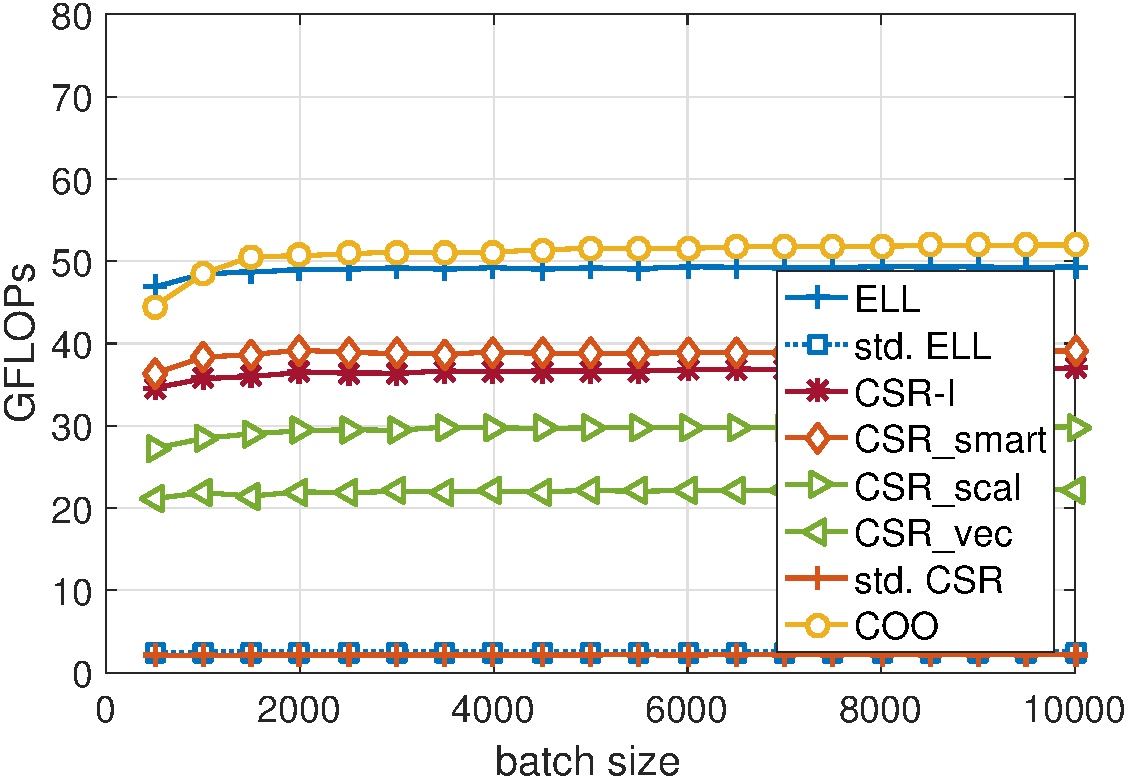
\includegraphics[width=.30\columnwidth]{plots/single_matrices/GFLOPS/cage8_GFLOPs}
&
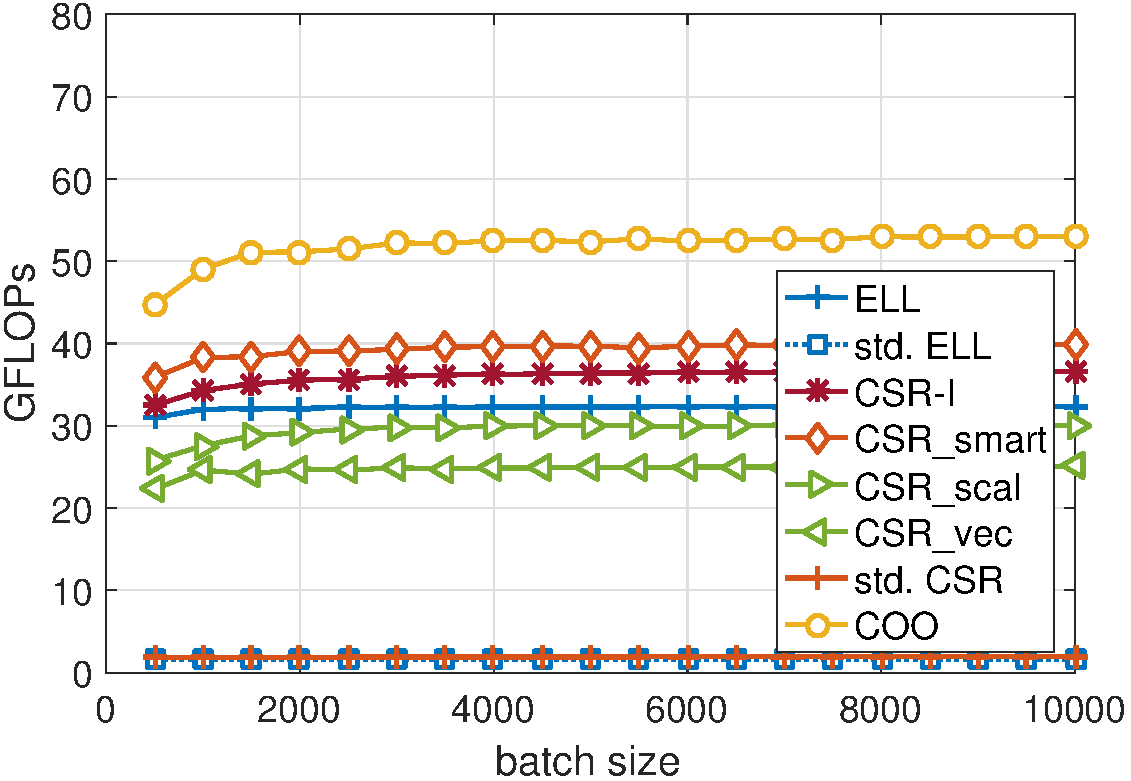
\includegraphics[width=.30\columnwidth]{plots/single_matrices/GFLOPS/can_838_GFLOPs}
&
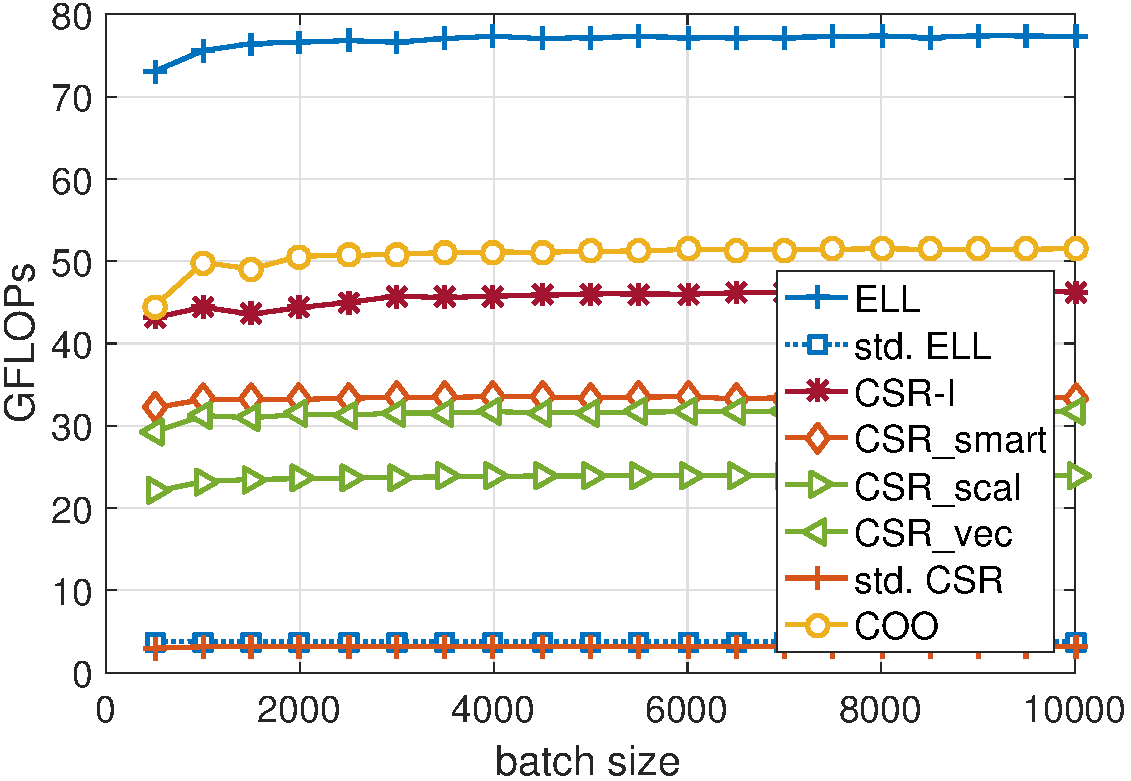
\includegraphics[width=.30\columnwidth]{plots/single_matrices/GFLOPS/dwt_992_GFLOPs}
\\
\hline
{\sc ex25} & {\sc ex27} & {\sc gr\_30\_30}\\
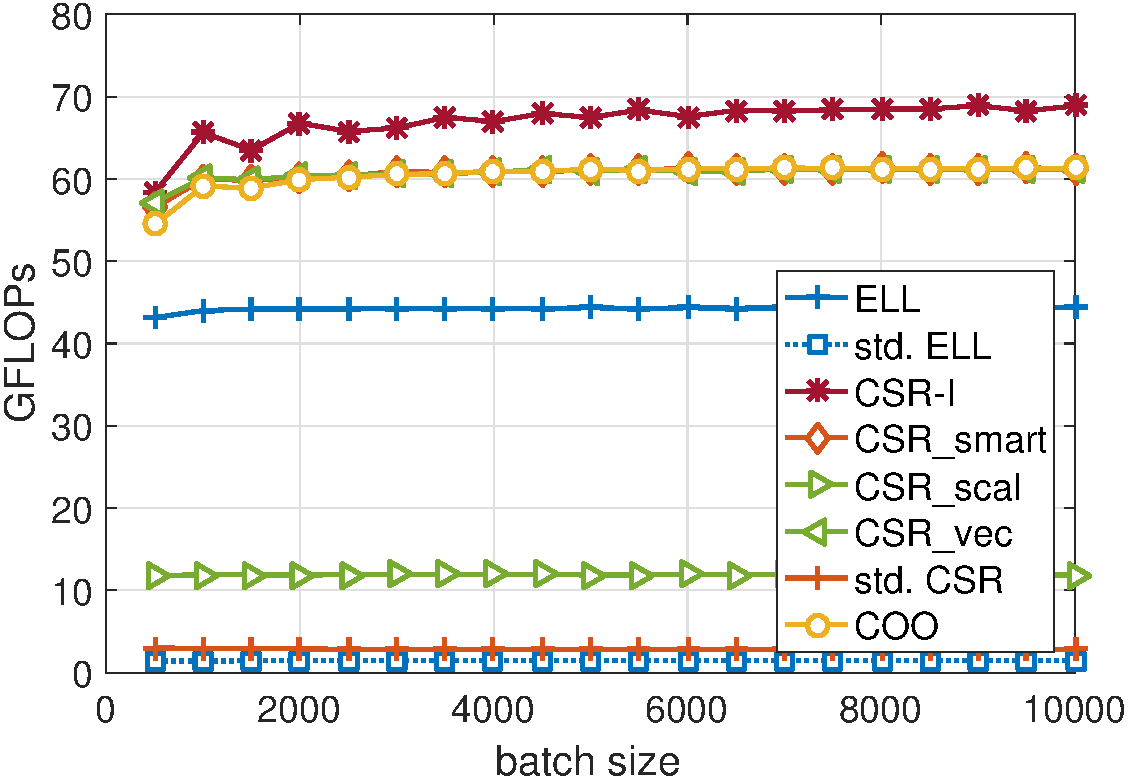
\includegraphics[width=.30\columnwidth]{plots/single_matrices/GFLOPS/ex2_GFLOPs}
&
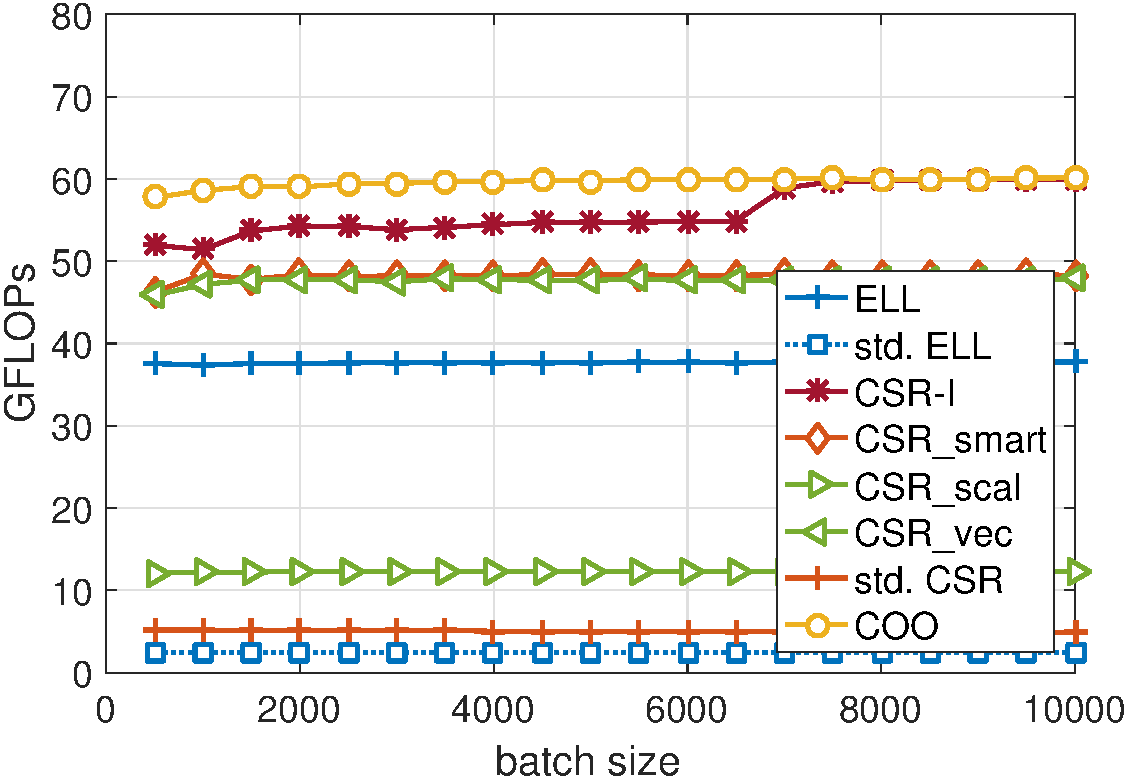
\includegraphics[width=.30\columnwidth]{plots/single_matrices/GFLOPS/ex27_GFLOPs}
&
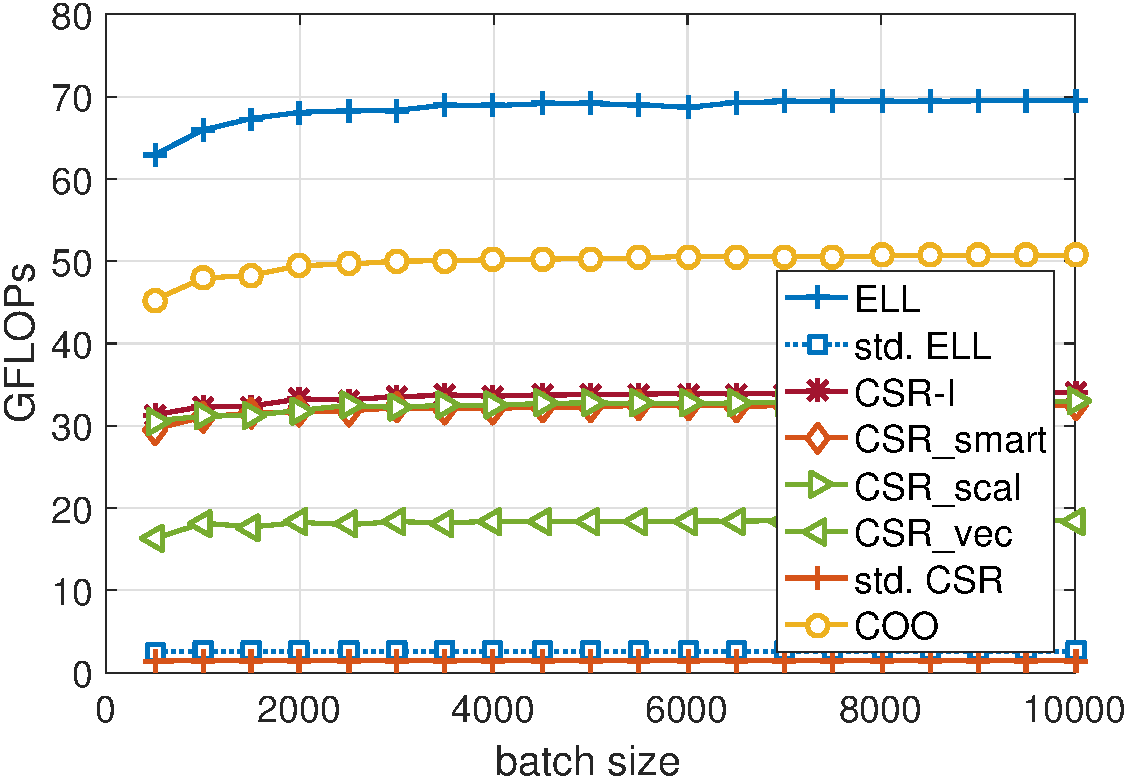
\includegraphics[width=.30\columnwidth]{plots/single_matrices/GFLOPS/gr_30_30_GFLOPs}
\\
\hline
{\sc mcfe} & {\sc msc} & {\sc nos3}\\
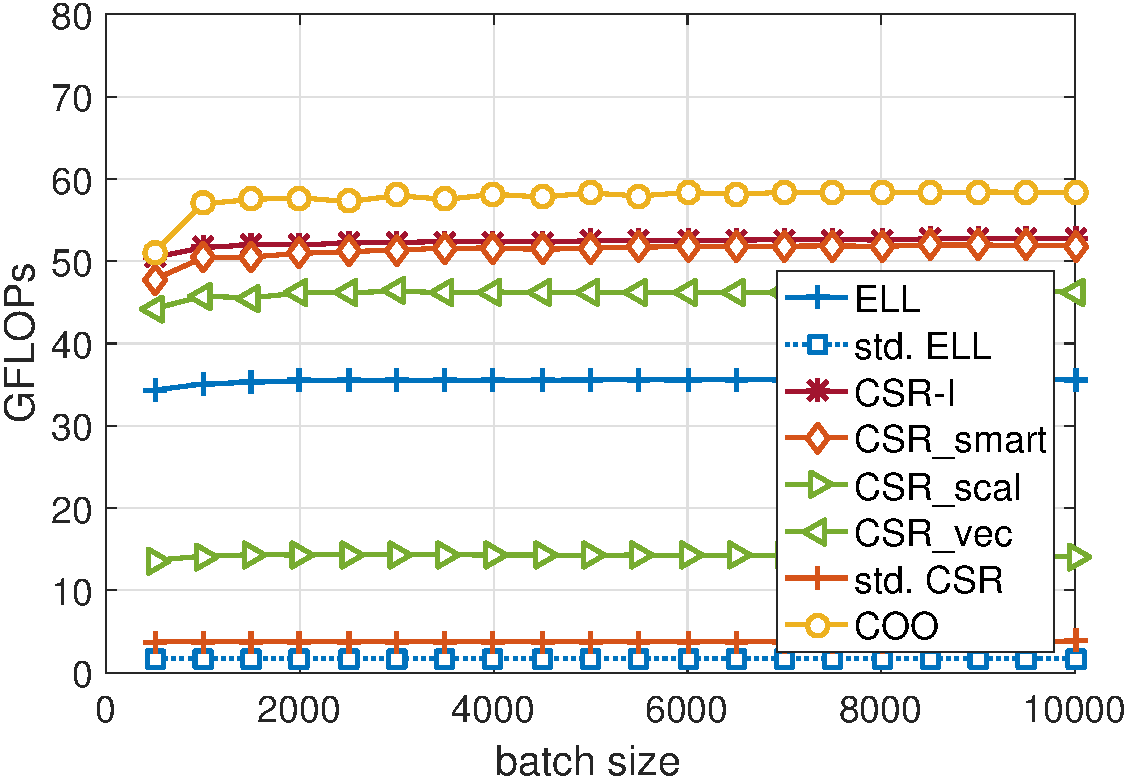
\includegraphics[width=.30\columnwidth]{plots/single_matrices/GFLOPS/mcfe_GFLOPs}
&
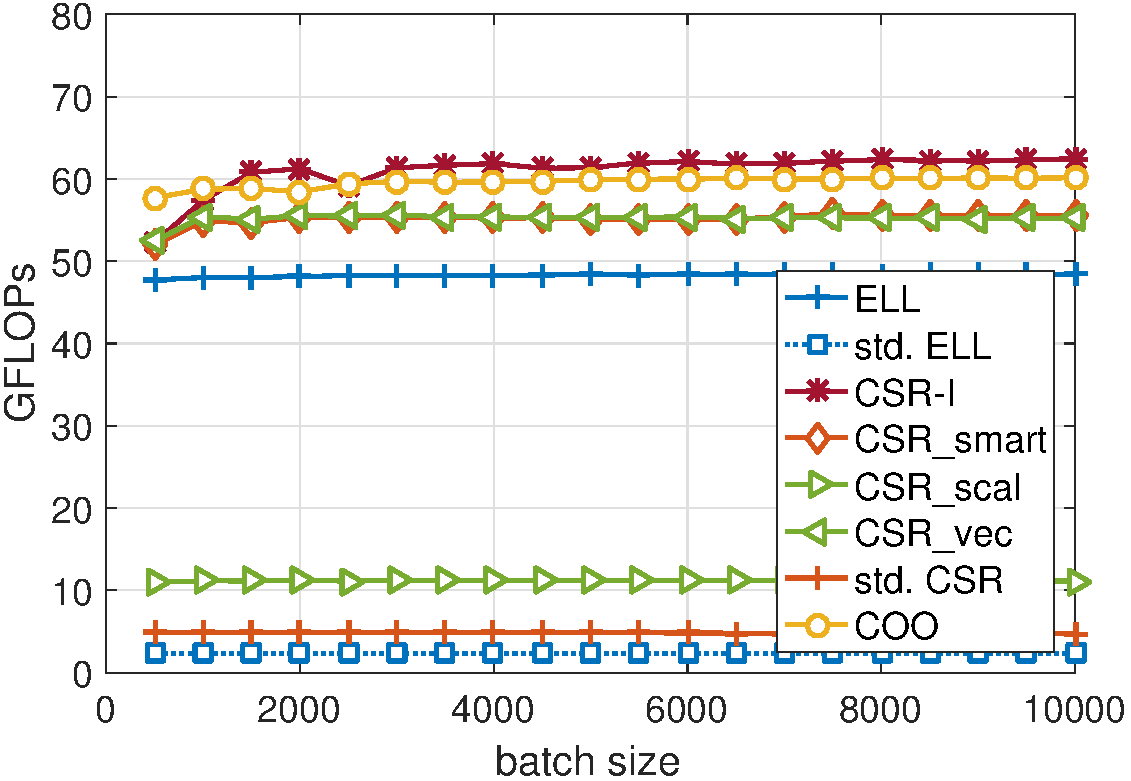
\includegraphics[width=.30\columnwidth]{plots/single_matrices/GFLOPS/msc00726_GFLOPs}
&
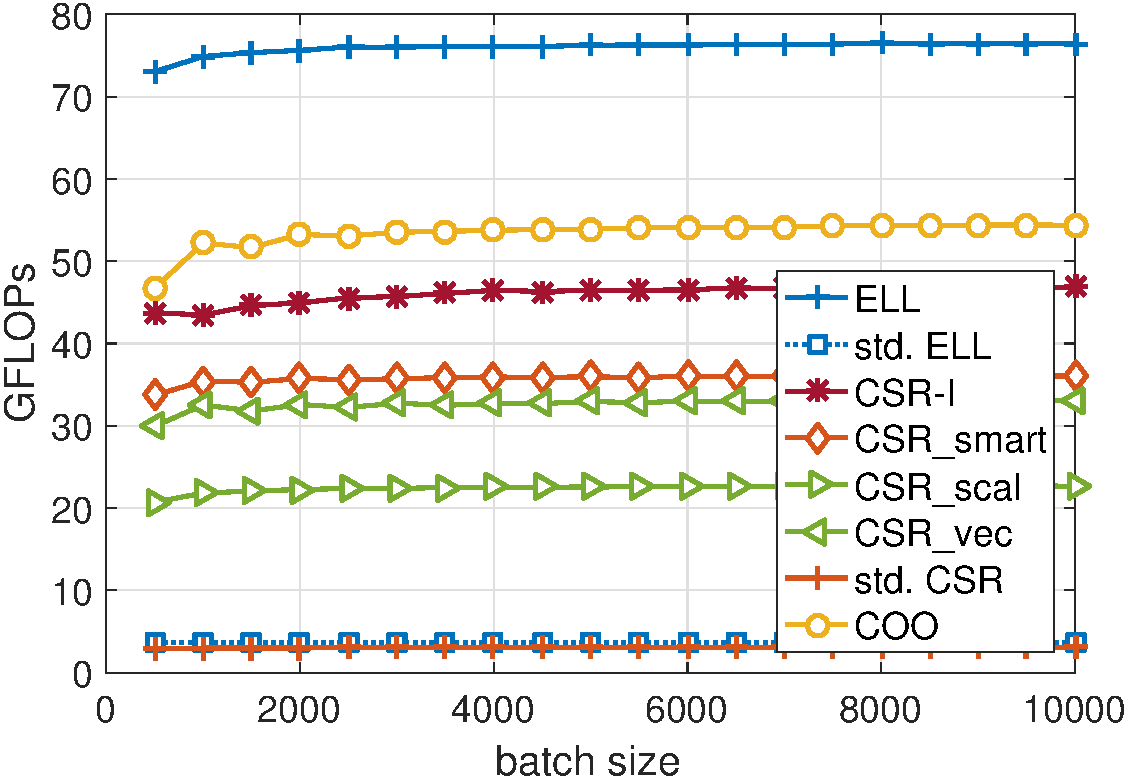
\includegraphics[width=.30\columnwidth]{plots/single_matrices/GFLOPS/nos3_GFLOPs}
\\
\hline
{\sc Si2} & {\sc rotor2} & {\sc west0989}\\
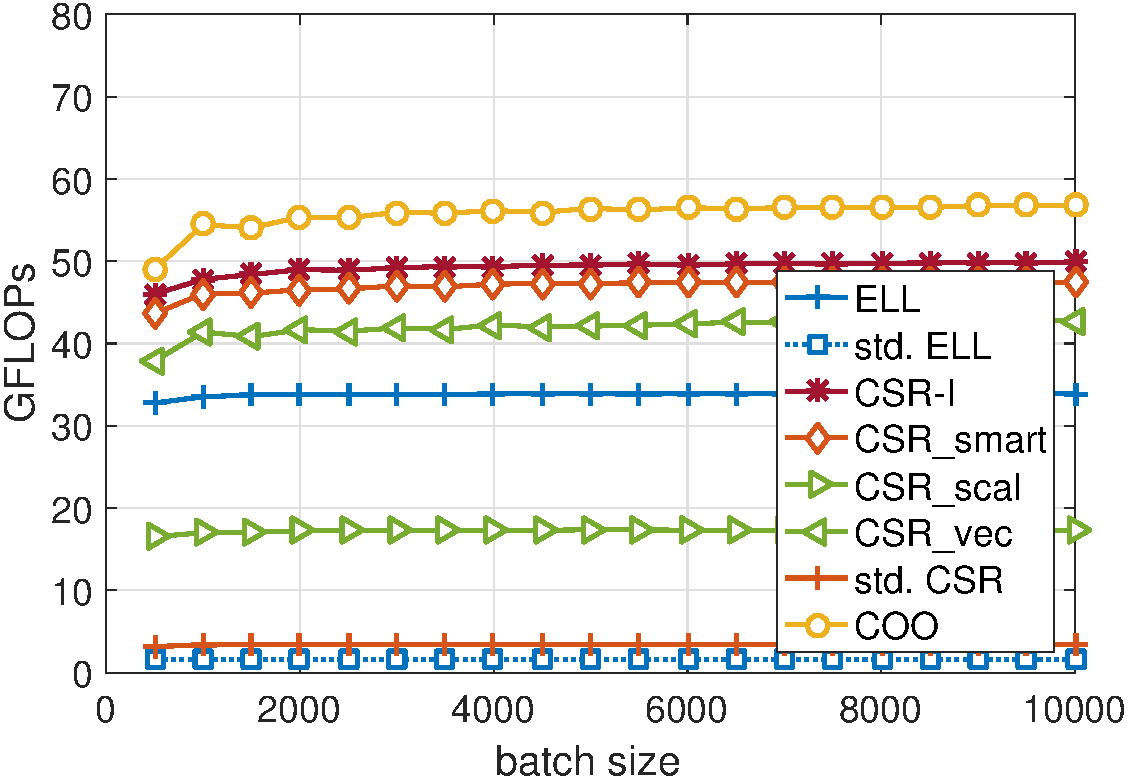
\includegraphics[width=.30\columnwidth]{plots/single_matrices/GFLOPS/Si2_GFLOPs}
&
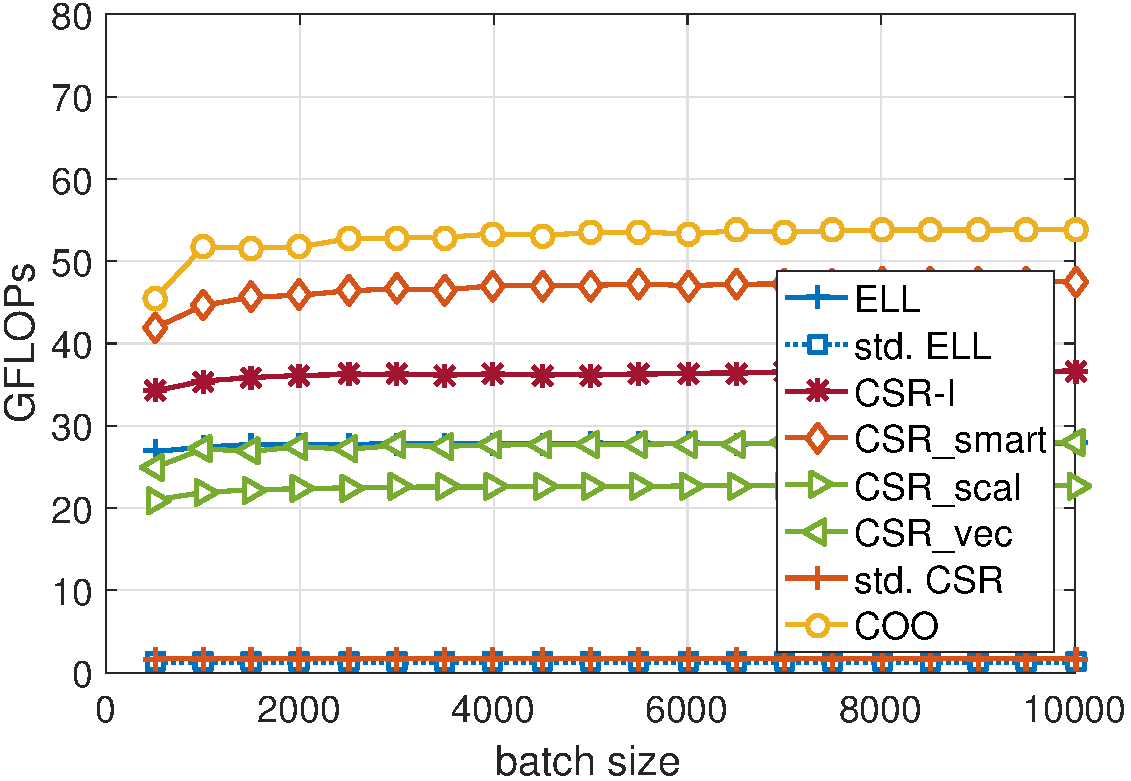
\includegraphics[width=.30\columnwidth]{plots/single_matrices/GFLOPS/rotor2_GFLOPs}
&
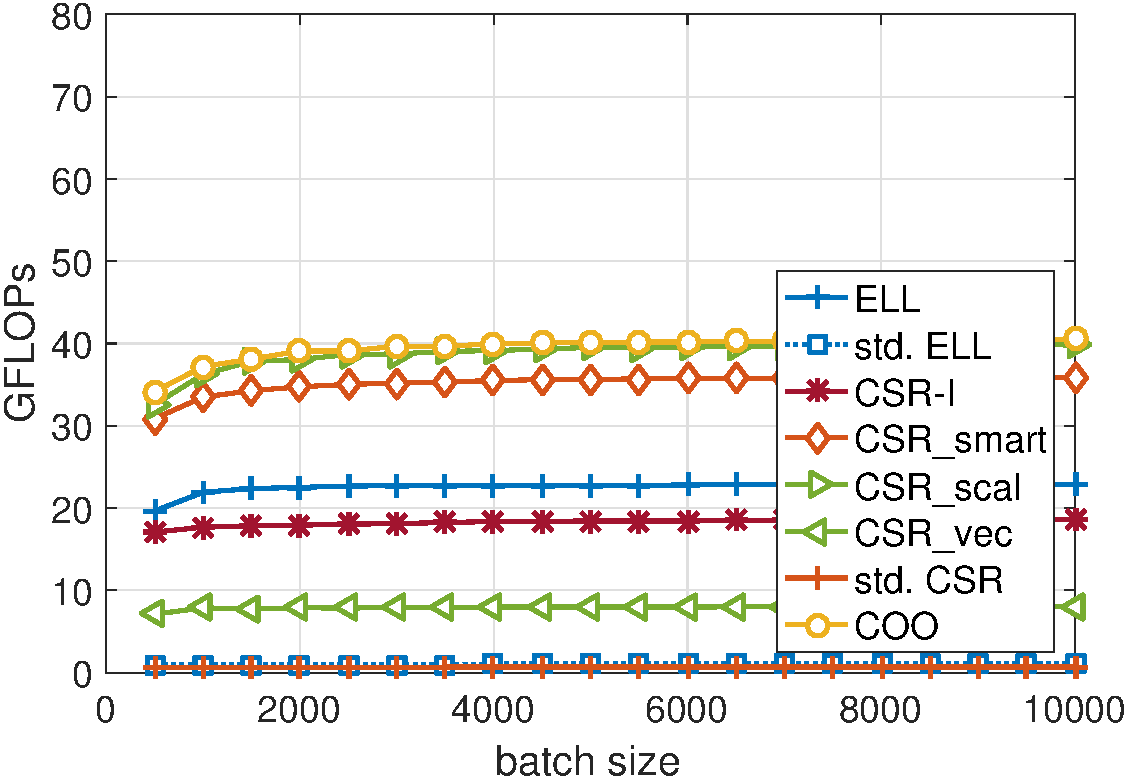
\includegraphics[width=.30\columnwidth]{plots/single_matrices/GFLOPS/west0989_GFLOPs}

\end{tabular}
\end{center}
\caption
[Performance of \spmv routines for homogeneous batches]
{Performance of the standard and the flexible batched \spmv routines 
for homogeneous batches.}
\label{2017-batched-spmv:fig:selectperf}
\end{figure}

